\section{Špecifikácia požiadavkov}

Účelom systému je zabezpečiť virtuálnu konferenciu. Webová aplikácia musí mať prvky redakčného systému, ktoré umožnia administrátorovi upravovať, pridávať a odoberať jej obsah. \\ \\

Účelom aplikácie bude zbieranie a sprostredkovávanie článkov vo forme virtuálneho časopisu. Aplikácia bude zobrazovať na webové rozhranie prehľad základných informácií o každom článku a to:
\begin{center}
\begin{itemize}
\item autora 
\item inštitúciu
\item názov
\item kľúčové slová
\item anotáciu
\item odkaz na plný text v PDF formáte
\end{itemize}
\end{center}

Aplikácia bude obsahovať vyhľadávanie v informáciách uložených v databáze. Vyhľadávanie bude možné podľa základných informácii okrem anotácie taktiež sa nebude vyhľadávať v samotnom texte článkov.\\ \\

Ku každému článku bude diskusia kde budu môcť užívatelia vyjadriť svoj názor k článku a budú mať možnosť reagovať na komentáre iných užívateľov. Diskusia bude rozvrstvená podla logickej náväznosti komentárov.\\ \\

Aplikácia bude rozlišovať užívateľov, ktorí k nej budu pristupovať. Každý užívateľ, ktorý sa neprihlási bude mať právomoci neregistrovaného užívateľa. Na registráciu bude k dispozícii formulár na vytváranie novích registorvaních užívateľov.\\ 

Administrátorský účet bude pridelený užívateľovi pri inicializačnom spustení webovej aplikácie. Prípadné ďalšie administrátorské účty musí vytvárať už existujúci administrátor.\\
Systém rozoznáva nasledovne užívateľské skupiny:
\begin{itemize}
 \item[\textbf{Administrátor}] - Administrátor bude mať možnosť manipulovať s obsahom stránok, spravovať užívateľov a má na starosti prvotnú konfiguráciu. V správe užívateľov bude potvrdzovať nové žiadosti o registráciu, bude môcť pozmeňovať údaje o užívateľovi, meniť ich role a blokovať účty.
\item[\textbf{Neregistrovaný užívateľ}] - Bude mať možnosť prehliadať zoznam uložených článkov, môže v nich vyhľadávať ale nemá prístup k plným textom článkov.
\item[\textbf{Registrovaný užívateľ}] - Bude mať všetky práva neregistrovaného užívateľa a naviac aj prístup k plným textom článkov z ročníka, pre ktorý zaplatil členský poplatok. Taktiež bude môcť za základný členský poplatok vložiť jeden článok. Bude si môcť upravovať informácie v profile a meniť pristupové heslo.
\item[\textbf{Redakčná rada}] - Bude mať možnosť stopnúť uverejnenie príspevku s odôvodnením jeho pozastavenia.
\item[\textbf{Recenzenti}] - Budú mať prístup k textom článkov v upraviteľnej podobe a k odovzdaným článkom majú možnosť pridávať recenzovanú verziu.
\end{itemize}

Aplikácia bude obsahovať radu notifikácii. Pri založení nového účtu bude zaslaná informácia administrátorovi so žiadosťou o jeho potvrdenie po overení zaplatenia členského poplatku.\\
Pri každom vložení nového článku registrovaným užívateľom budú vybraný a oboznámený o tomto článku recenzenti, ktorých úlohou bude článok recenzovať.\\
Registrovaný užívatelia si môžu povoliť oznámenie o nových zverejnených článkoch cez mail a pre všetkých užívateľov bude k dispozícii RSS zdroj. \\
Po dovŕšení limitu na zostavenie čísla časopisu bude o tom informovaná redakčná rada a administrátor. \\ \\

Pravidelne bude spúšťané zálohovanie databázy, ako aj uložených plných textov článkov, ktoré budú slúžiť na obnovenie dát v prípade poruchy. Kompletné zálohy budú ukladané na predurčené uložisko. \\ \\

Redakčné prvky systému umožnia administrátorovi upravovať a dopĺňať webové rozhranie systému. Bude mať možnosť meniť logo portálu, texty na stránkach, pridávať a zneplatňovať nové stránky. \\
Všetky zmeny rozloženia stránok sa budú prejavovať v štruktúre menu stránky, ktoré bude najviac 2 úrovňové. Stránky budu môcť byť doplňované do ktorejkoľvek úrovne menu.\\ \\

Webové rozhranie bude umožňovať zmenu vzhľadu pomocou dodávaných tém. Aplikácia bude vyhotovená s jednou štandardnou témou a s témou pre postihnutých. \\
Téma sa bude pre registrovaných užívateľov ukladať do ich profilu.\\ \\

Nevyhnutná konfigurácia hotovej distribúcie prebehne pri jeho prvom spustení. Vytvori sa tu administrátorské konto a všetky nevyhnutné nastavenia aplikácie. \\
Celý nasledujúci beh systému bude automaticky a všetky prípadne zmeny nastavenia a obsahu sa budu diať cez webové rozhranie administrátora. \\ \\

Webové rozhranie bude prehľadne a funkcionálne, zamerane na rýchle dosiahnutie požadovaných informácií. Každá stránka musí obsahovať tieto prvky:
\begin{center}
\begin{itemize}
\item logo a základne údaje o organizácii zriaďujúcej virtuálnu konferenciu
\item menu stránok webového rozhrania
\item ak je užívateľ neprihlásený -- možnosť prihlásiť sa do systému
\item ak je užívateľ prihlásený -- meno užívateľa a voľbu na odhlásenie sa
\end{itemize}
\end{center}

Informácie o uložených článkoch sa budu zobrazovať do prehľadného výpisu obsahujúceho základné informácie. Záznamy sa budú zobrazovať pre aktuálny rok. Staršie ročníky budú uložené v archíve. \\
Záznamy pre aktuálny ročník budu chronologicky usporiadané od najnovších po najstaršie. Archív bude usporiadaný podľa rokov a bude rovnako zoradený ako aktuálny ročník. Parameter zoraďovanie bude môcť užívateľ pozmeniť na meno, inštitúciu, názov a dátum. Taktiež bude možnosť zmeniť vzostupnosť alebo zostupnosť usporiadania.\\
V prípade, že záznamov bude viac ako limit zobrazenia na jednu stránku, zoznam sa stane viac stranovým. Užívateľ si bude môcť zvoliť koľko záznamov chce na jedne krát zobraziť.\\ \\

Rozhranie vyhľadávania bude čo najjednoduchšie. Bude poskytovať voľby na určenie kategórie, v ktorej sa bude vyhľadávať:
\begin{center}
\begin{itemize}
\item meno, inštitúcia, názov
\item kľúčové slová
\item ročník 
\end{itemize}
\end{center}

\begin{center}
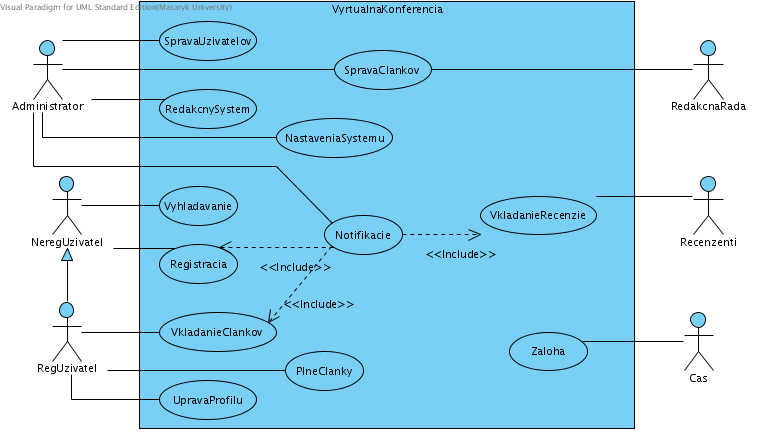
\includegraphics[width=\linewidth]{VyrtualnaKonferencia.png}
 % Use_Case_Diagram1.png: 742x436 pixel, 72dpi, 26.18x15.38 cm, bb=0 0 742 436
\textit{Use case diagram virtuálnej konferencie.}
\end{center}



